% =========================================================================
% SENDA — educational guide (public edition of the LATTIMEX repository, 2026-09-30)
% English translation of guia_senda.tex. SPDX-License-Identifier: CC-BY-4.0
% Build: pdflatex senda_guide_en && bibtex senda_guide_en
% Then: pdflatex senda_guide_en (twice to resolve references).
% Figure data and macros in datos/; figures in figuras/.
% =========================================================================
\documentclass[11pt,a4paper]{article}

\usepackage[T1]{fontenc}
\usepackage{lmodern}
\usepackage[english]{babel}
\usepackage[margin=2.4cm]{geometry}
\usepackage{microtype}
\usepackage{amsmath,amssymb}
\usepackage{booktabs}
\usepackage{array}
\usepackage{graphicx}
\usepackage{float}
\usepackage[font=small,labelfont=bf]{caption}
\usepackage{enumitem}
\usepackage[dvipsnames]{xcolor}
\usepackage{tikz}
\usetikzlibrary{arrows.meta,positioning,decorations.pathreplacing,calc,shapes.geometric}
\usepackage{pgfplots}
\pgfplotsset{compat=1.18}
\usepackage[most]{tcolorbox}
\usepackage{algorithm}
\usepackage{algpseudocode}
\usepackage{url}
\usepackage[colorlinks=true,linkcolor=MidnightBlue,citecolor=OliveGreen,urlcolor=MidnightBlue]{hyperref}

\algrenewcommand\algorithmicrequire{\textbf{Input:}}
\algrenewcommand\algorithmicensure{\textbf{Output:}}
\newcommand{\IfReturn}[2]{\State \textbf{if} #1 \textbf{then return} #2}

% --- Teaching boxes -------------------------------------------------------
\definecolor{sendaink}{RGB}{19,34,31}
\definecolor{sendared}{RGB}{210,75,50}
\definecolor{sendagreen}{RGB}{11,131,96}
\newtcolorbox{ideaclave}[1][]{enhanced,breakable,colback=sendagreen!6,colframe=sendagreen!70!black,
  fonttitle=\bfseries,title={Key idea#1},left=6pt,right=6pt,top=4pt,bottom=4pt}
\newtcolorbox{ejemplo}[1][]{enhanced,breakable,colback=MidnightBlue!4,colframe=MidnightBlue!70,
  fonttitle=\bfseries,title={Worked example#1},left=6pt,right=6pt,top=4pt,bottom=4pt}
\newtcolorbox{leccion}[1][]{enhanced,breakable,colback=sendared!6,colframe=sendared!85!black,
  fonttitle=\bfseries,title={Methodological lesson#1},left=6pt,right=6pt,top=4pt,bottom=4pt}
\newtcolorbox{reproducir}[1][]{enhanced,breakable,colback=gray!6,colframe=gray!60!black,
  fonttitle=\bfseries,title={To reproduce#1},left=6pt,right=6pt,top=4pt,bottom=4pt}
\newtcolorbox{ficha}[1]{enhanced,breakable,colback=white,colframe=sendaink!70,
  fonttitle=\bfseries,title={#1},left=6pt,right=6pt,top=4pt,bottom=4pt}

\newcommand{\senda}{SENDA}
\newcommand{\pp}{\,pp}
\newcommand{\tsl}[1]{\texttt{\small #1}}

% generado por preparar_datos.py
\newcommand{\cinfABEa}{0}
\newcommand{\cfeABEa}{100}
\newcommand{\cgfABEa}{81.008}
\newcommand{\cnfABEa}{63}
\newcommand{\cgrABEa}{81.008}
\newcommand{\cinfABEb}{105}
\newcommand{\cfeABEb}{83}
\newcommand{\cgfABEb}{4.671}
\newcommand{\cnfABEb}{62}
\newcommand{\cgrABEb}{4.577}
\newcommand{\cinfABEc}{321}
\newcommand{\cfeABEc}{49}
\newcommand{\cgfABEc}{3.475}
\newcommand{\cnfABEc}{51}
\newcommand{\cgrABEc}{0.238}
\newcommand{\cinfABEd}{0}
\newcommand{\cfeABEd}{100}
\newcommand{\cgfABEd}{0.319}
\newcommand{\cnfABEd}{63}
\newcommand{\cgrABEd}{0.319}
\newcommand{\cinfABEe}{0}
\newcommand{\cfeABEe}{100}
\newcommand{\cgfABEe}{0.243}
\newcommand{\cnfABEe}{63}
\newcommand{\cgrABEe}{0.243}
\newcommand{\cinfABEf}{0}
\newcommand{\cfeABEf}{100}
\newcommand{\cgfABEf}{0.115}
\newcommand{\cnfABEf}{63}
\newcommand{\cgrABEf}{0.115}
\newcommand{\cnABE}{63}
\newcommand{\cgABEa}{81.008}
\newcommand{\cbABEa}{0}
\newcommand{\cgABEb}{18.972}
\newcommand{\cbABEb}{0}
\newcommand{\csABEb}{76.7}
\newcommand{\cgABEc}{46.181}
\newcommand{\cbABEc}{0}
\newcommand{\csABEc}{-33.6}
\newcommand{\cgABEd}{0.319}
\newcommand{\cbABEd}{31}
\newcommand{\csABEd}{56.7}
\newcommand{\cgABEe}{0.243}
\newcommand{\cbABEe}{31}
\newcommand{\csABEe}{0.1}
\newcommand{\cgABEf}{0.115}
\newcommand{\cbABEf}{37}
\newcommand{\csABEf}{0.2}
\newcommand{\cpeorABE}{0}
\newcommand{\ctotABE}{630}
\newcommand{\cinfXa}{0}
\newcommand{\cfeXa}{100}
\newcommand{\cgfXa}{25.786}
\newcommand{\cnfXa}{41}
\newcommand{\cgrXa}{25.786}
\newcommand{\cinfXb}{119}
\newcommand{\cfeXb}{71}
\newcommand{\cgfXb}{6.262}
\newcommand{\cnfXb}{39}
\newcommand{\cgrXb}{6.478}
\newcommand{\cinfXc}{236}
\newcommand{\cfeXc}{42}
\newcommand{\cgfXc}{5.244}
\newcommand{\cnfXc}{32}
\newcommand{\cgrXc}{4.129}
\newcommand{\cinfXd}{0}
\newcommand{\cfeXd}{100}
\newcommand{\cgfXd}{4.971}
\newcommand{\cnfXd}{41}
\newcommand{\cgrXd}{4.971}
\newcommand{\cinfXe}{0}
\newcommand{\cfeXe}{100}
\newcommand{\cgfXe}{4.459}
\newcommand{\cnfXe}{41}
\newcommand{\cgrXe}{4.459}
\newcommand{\cinfXf}{0}
\newcommand{\cfeXf}{100}
\newcommand{\cgfXf}{4.121}
\newcommand{\cnfXf}{41}
\newcommand{\cgrXf}{4.121}
\newcommand{\cnX}{41}
\newcommand{\cgXa}{25.786}
\newcommand{\cbXa}{0}
\newcommand{\cgXb}{14.453}
\newcommand{\cbXb}{0}
\newcommand{\csXb}{52.3}
\newcommand{\cgXc}{19.508}
\newcommand{\cbXc}{0}
\newcommand{\csXc}{-23.3}
\newcommand{\cgXd}{4.971}
\newcommand{\cbXd}{0}
\newcommand{\csXd}{67.1}
\newcommand{\cgXe}{4.459}
\newcommand{\cbXe}{0}
\newcommand{\csXe}{2.4}
\newcommand{\cgXf}{4.121}
\newcommand{\cbXf}{0}
\newcommand{\csXf}{1.6}
\newcommand{\cpeorX}{0}
\newcommand{\ctotX}{410}
\newcommand{\trazaInst}{A-n80-k10}
\newcommand{\trazaBKS}{1763}
\newcommand{\trazaA}{3180 (80.37\,\%)}
\newcommand{\trazaB}{1827 (3.63\,\%)}
\newcommand{\trazaC}{1865 (5.79\,\%)}
\newcommand{\trazaD}{1783 (1.13\,\%)}
\newcommand{\trazaE}{1766 (0.17\,\%)}
\newcommand{\trazaF}{1766 (0.17\,\%)}


\title{\textbf{SENDA: vehicle routing with single-trajectory search,\\ explained and measured honestly}\\[0.4em]
\large An educational guide to the LATTIMEX routing core: how it works, how it was evaluated\\ and how to try it on your computer}
\author{Erick Martínez\\
\small LATTIMEX · independent research · Querétaro, Mexico\\
\small \texttt{contacto@lattimex.com} · \texttt{https://lattimex.com}}
\date{September 30, 2026\\[0.3em]\small English translation of the Spanish original}

\hypersetup{
  pdftitle={SENDA: an educational guide to the LATTIMEX routing core},
  pdfauthor={Erick Martínez (LATTIMEX)},
  pdfsubject={Educational guide under Creative Commons Attribution 4.0 International (CC BY 4.0)},
  pdfkeywords={CVRP, ALNS, LATTIMEX, CC BY 4.0}
}

% Notice on the first page, without changing the text area.
\makeatletter
\def\ps@licenciaguia{%
  \let\@oddhead\@empty
  \let\@evenhead\@empty
  \def\@oddfoot{\vtop{\offinterlineskip%
    \hbox to\textwidth{\hfil\thepage\hfil}%
    \vskip5pt
    \hbox to\textwidth{\hfil\scriptsize\textcopyright{} 2026 Erick Martínez (LATTIMEX).
      CC BY 4.0: \url{https://creativecommons.org/licenses/by/4.0/}\hfil}}}%
  \let\@evenfoot\@oddfoot
}
\makeatother

\begin{document}
\maketitle
\thispagestyle{licenciaguia}

\begin{abstract}
\noindent\textbf{In a nutshell.} Assigning deliveries to vehicles and deciding the order of visits is
a classic optimization problem that cannot be solved exactly at large scale: heuristics are used
instead, programs that find very good solutions in little time. This guide opens one of them, the
routing core of the LATTIMEX engine, piece by piece, and shows how to measure its quality without
fooling yourself. At the end, the reader can install the engine, which is open source (MIT), and
check the results on their own computer.

\smallskip
\noindent This document explains, from scratch and with worked examples, how \senda{} works and how it
was evaluated. \senda{} is a solver for the capacitated vehicle routing problem (CVRP). The solver
follows a single search trajectory: it builds an initial solution, improves it with granular local
search, restructures it with an adaptive large neighborhood search (ALNS), refines it with segment
moves and SWAP*, and splits its time among two or three variants chosen from the features of the
instance (a portfolio of configurations). For each component the guide explains what it is, why it
matters and how much it contributes. A cascade experiment measures the quality available after each
stage: on A/B/E the mean gap goes from \cgABEa\,\% after construction to \cgABEf\,\% with the full
portfolio, and on X from \cgXa\,\% to \cgXf\,\%. With a frozen contract, 10 external replicates, the
same clock for all methods and independent verification, \senda{} obtains on 60 A/B/E instances a gap
of 0.111\,\% versus 0.004\,\% for HGS-CVRP (it ties on 37 and HGS is better on 23). On 41 X instances
it obtains 4.119\,\%, versus 1.450\,\% for HGS and 0.758\,\% for FILO2. The document includes a case
study on a verification error and its correction.
\end{abstract}

\noindent\textbf{Keywords:} vehicle routing; CVRP; ALNS; granular search; SWAP*;
reproducible evaluation; teaching optimization.

\tableofcontents
\newpage

% =========================================================================
\section*{How to read this document}
\addcontentsline{toc}{section}{How to read this document}

The text is aimed at students, logistics engineers and anyone who wants to understand a modern
routing heuristic and the right way to measure its quality. No prior experience with metaheuristics
is required: basic notions of graphs, probability and statistics are enough.

\begin{itemize}[leftmargin=1.5em]
\item Sections~\ref{sec:cvrp} and~\ref{sec:senda} present the problem and what SENDA is.
\item Sections~\ref{sec:flujo}--\ref{sec:cascada} are the teaching core: they describe each
component, how the solution passes from one to the next and how much quality each step adds.
\item Section~\ref{sec:complejidad} introduces big-$O$ notation and estimates how much each component
costs.
\item Section~\ref{sec:evaluar} explains how to evaluate a heuristic without fooling yourself.
\item Sections~\ref{sec:resultados} and~\ref{sec:caso} present the results and a case study on a real
error.
\item Section~\ref{sec:pruebalo} explains how to install the engine and repeat the measurements on
your computer.
\end{itemize}

\paragraph{What you will learn.} (1) What the CVRP is and why it is solved with heuristics; (2) how a
routing solution is built, improved and diversified, with an example for each component; (3) how to
estimate with big-$O$ notation how much each component costs and why that limits quality under a
fixed clock; (4) how to design a fair comparison (same clock, replicates, independent verification,
paired statistics); (5) how a verification error can manufacture ``wins'' and how to detect it; and
(6) how to go from an academic solver to an engine that plans real routes with three-dimensional
loading.

The boxes serve four purposes:

\begin{ideaclave}
Summarizes the concept that should not be forgotten.
\end{ideaclave}
\begin{ejemplo}
Solves a small calculation, step by step and with concrete numbers.
\end{ejemplo}
\begin{leccion}
Describes a possible error, or one that actually happened in this project, and how to avoid it.
\end{leccion}
\begin{reproducir}
Gives the SHA-256 fingerprints of the artifacts behind a figure and how to repeat the measurement.
\end{reproducir}

\paragraph{About this edition.} This guide accompanies the public LATTIMEX repository. The programs
used for comparison (HGS-CVRP, FILO2 and the campaign scripts) are not part of the repository: they
are described here so that the comparison is transparent, and Section~\ref{sec:pruebalo} explains
how to repeat it with copies obtained from their official sources. Raw data, contracts and logs are
kept in the author's archive; each figure cites the SHA-256 fingerprint of the artifact behind it.
This edition includes the correction of the A/B/E comparison (Section~\ref{sec:caso}). It is a
translation of the Spanish original (\tsl{guia\_senda.pdf}); in case of discrepancy, the original
prevails. Instance names, configuration names and identifiers in the code are kept as they appear
in the original.

% =========================================================================
\section{Introduction}
\label{sec:intro}

Every day, parcel, distribution and service companies decide which vehicle visits which customers
and in what order. That decision, repeated thousands of times, is the \emph{capacitated vehicle
routing problem} (CVRP), first formulated by Dantzig and Ramser~\cite{dantzig1959}. Its statement is
short, but the number of possible solutions grows explosively with the number of customers. That is
why, in practice, it is solved with \emph{heuristics}: algorithms that find very good solutions in
seconds, even though they cannot guarantee that they are optimal.

The state of the art in heuristics is dominated by hybrid genetic search
HGS-CVRP~\cite{vidal2012,vidal2022hgs} and by very fast solvers such as FILO2~\cite{accorsi2023}.
This work does not aim to beat them. Its goal is to build a \emph{compact and auditable} solver ---a
single search trajectory, with no population of solutions and no crossover--- and to answer three
questions with reproducible evidence:

\begin{enumerate}[label=\textbf{Q\arabic*.}]
\item What does each component of the solver do, and how much quality does it add?
\item What final quality does it reach, with the same time as the reference solvers, on small (A/B/E)
and large (X) instances?
\item What is learned when the evaluation protocol itself contains an error?
\end{enumerate}

\paragraph{Contributions.}
(1) A complete description of \senda{}, component by component, with pseudocode and numerical
examples.
(2) A measurement of the quality each stage adds, complementary to the classic ablation.
(3) An evaluation protocol with a frozen contract, replicates, independent verification and
per-instance inference.
(4) An honest comparison against HGS and FILO2 that delimits where the lightweight architecture is
competitive and where it is not.
(5) A case study on a verification error and its correction.

% =========================================================================
\section{The CVRP in ten minutes}
\label{sec:cvrp}

\subsection{Definition}
A CVRP instance has a depot, identified as node $0$; a set of customers $V=\{1,\dots,n\}$, each with
a demand $q_i>0$; a vehicle capacity $Q$; and a distance $d(i,j)$ between every pair of points. A
\emph{route} leaves the depot, visits a sequence of customers and returns to the depot. A
\emph{solution} is a set of routes that satisfies three conditions:
\begin{enumerate}[label=(\roman*)]
\item every customer is visited exactly once (\emph{coverage});
\item the total demand of each route does not exceed $Q$ (\emph{capacity});
\item the number of routes does not exceed the available fleet $k$, when the instance fixes it
(\emph{fleet}).
\end{enumerate}
The objective is to minimize the total distance traveled:
\begin{equation}
C(S) \;=\; \sum_{r\in S}\;\sum_{(i,j)\in r} d(i,j).
\label{eq:costo}
\end{equation}

\begin{figure}[H]
\centering
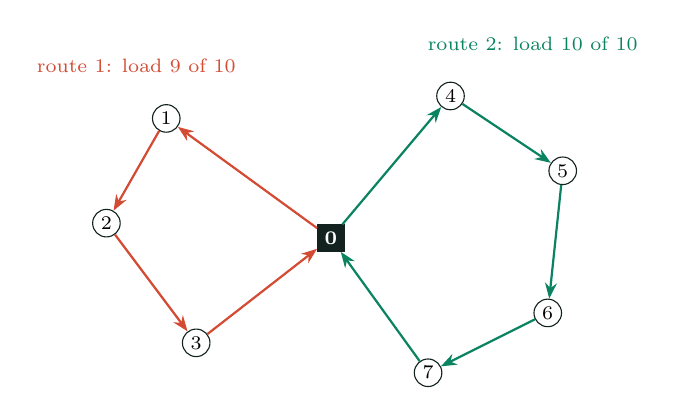
\begin{tikzpicture}[scale=0.95,
  cli/.style={circle,draw=sendaink,fill=white,inner sep=1.4pt,font=\scriptsize},
  dep/.style={rectangle,draw=sendaink,fill=sendaink,text=white,inner sep=2.5pt,font=\scriptsize\bfseries}]
\node[dep] (D) at (0,0) {0};
\node[cli] (a) at (-2.2,1.6) {1}; \node[cli] (b) at (-3.0,0.2) {2}; \node[cli] (c) at (-1.8,-1.4) {3};
\node[cli] (e) at (1.6,1.9) {4}; \node[cli] (f) at (3.1,0.9) {5}; \node[cli] (g) at (2.9,-1.0) {6};
\node[cli] (h) at (1.3,-1.8) {7};
\foreach \u/\v in {D/a,a/b,b/c,c/D} \draw[-{Stealth[length=2mm]},thick,sendared] (\u)--(\v);
\foreach \u/\v in {D/e,e/f,f/g,g/h,h/D} \draw[-{Stealth[length=2mm]},thick,sendagreen] (\u)--(\v);
\node[font=\scriptsize,sendared] at (-2.6,2.3) {route 1: load 9 of 10};
\node[font=\scriptsize,sendagreen] at (2.7,2.6) {route 2: load 10 of 10};
\end{tikzpicture}
\caption{Solution of a small CVRP with 7 customers, capacity $Q=10$ and fleet $k=2$. Every customer is
visited only once and no route exceeds the capacity.}
\label{fig:cvrp}
\end{figure}

\subsection{How quality is measured: BKS and gap}
For the CVRPLIB reference instances~\cite{cvrplib} the \emph{best known solution} (BKS) is known; many
of them are certified as optimal~\cite{queiroga2021}. The quality of a heuristic is measured with the
\emph{gap}, the relative difference between its cost and the BKS:
\begin{equation}
\mathrm{gap}(S) \;=\; 100\cdot\frac{C(S)-C_{\mathrm{BKS}}}{C_{\mathrm{BKS}}}\ \text{(\%)}.
\label{eq:gap}
\end{equation}

\begin{ejemplo}[: computing a gap]
On instance \tsl{B-n51-k7} the BKS is 1032 and uses $k=7$ vehicles. If a solver delivers a solution
of cost 1040 with 7 routes, its gap is $100\cdot(1040-1032)/1032 = 0.78$\,\%. If it delivers one of
cost 1032, its gap is 0\,\%: it reached the BKS.
\end{ejemplo}

\begin{ideaclave}[: a negative gap is an alarm]
If the BKS is certified as optimal, \emph{no} correct solver can obtain a negative gap. A negative gap
means that the solution violates some constraint ---almost always the fleet constraint--- or that the
verification is wrong. Section~\ref{sec:caso} shows that this happened in this project.
\end{ideaclave}

\subsection{The benchmarks}
\begin{itemize}[leftmargin=1.5em]
\item \textbf{A, B and E} (Augerat and Christofides~\cite{augerat1995,christofides1969}): 63 classic
instances with 12 to 100 customers and a fixed fleet. The name gives the size and the fleet:
\tsl{A-n32-k5} has 32 nodes (31 customers and the depot) and 5 vehicles.
\item \textbf{X} (Uchoa et al.~\cite{uchoa2017}): large and more varied instances. 41 of them are used
here, with 199 to 428 customers and a free fleet. In X, the number $k$ in the name is a reference and
not a constraint.
\end{itemize}

% =========================================================================
\section{What SENDA is: one search trajectory per run}
\label{sec:senda}

SENDA (\emph{Single-trajectory ENgine with Destroy-and-repair Adaptive search}; in Spanish,
\emph{senda} means ``path'') is the routing core of the LATTIMEX engine. Its design trait is the one
that gives it its name: it follows \textbf{a single search trajectory per run}. Within each run there
is at all times one current solution ---with all its routes--- that is partially destroyed, repaired
and improved; there is no population of solutions crossed with one another, as in the
state-of-the-art genetic algorithms for the CVRP (for example, Vidal's
HGS-CVRP~\cite{vidal2022hgs}).

The decision has practical advantages that matter in a production engine: the path of the solution
can be followed step by step and explained (Section~\ref{sec:flujo}); effort is split among a few
stages with an explicit clock; and parallelism is obtained with a portfolio of independent
trajectories. The final choice among its candidates is deterministic; since the budget of each run is
wall-clock time and depends on the number of threads, the candidates ---and therefore the answer---
may vary between computers. The cost is also clear, and this guide measures it: on the pure CVRP,
with the same clock, a well-tuned population algorithm is still more accurate
(Section~\ref{sec:resultados}).

SENDA combines published ideas ---ALNS~\cite{ropke2006}, granular
neighborhoods~\cite{toth2003granular}, penalized infeasibility and the SWAP*
neighborhood~\cite{vidal2022hgs}--- in an original implementation. The contribution of this
implementation lies in how they are put together: the configuration selector driven by instance
features, the portfolio of arms with a shared clock and, in the LATTIMEX engine, the integration with
three-dimensional load placement, fixed-fleet mediation and the unloading plan by door.

% =========================================================================
\section{Map of the solver: how a solution flows}
\label{sec:flujo}

Before studying each component it helps to see the whole path. A single object circulates in
\senda{}: a \emph{solution}, which is a list of routes together with its cost, the load of each route
and a flag that says whether it is feasible. Each component receives a solution and delivers
another, usually shorter; some may pass through infeasible solutions while they work, but what they
deliver at the end is feasible. Figure~\ref{fig:flujo} shows that path.

\begin{figure}[H]
\centering
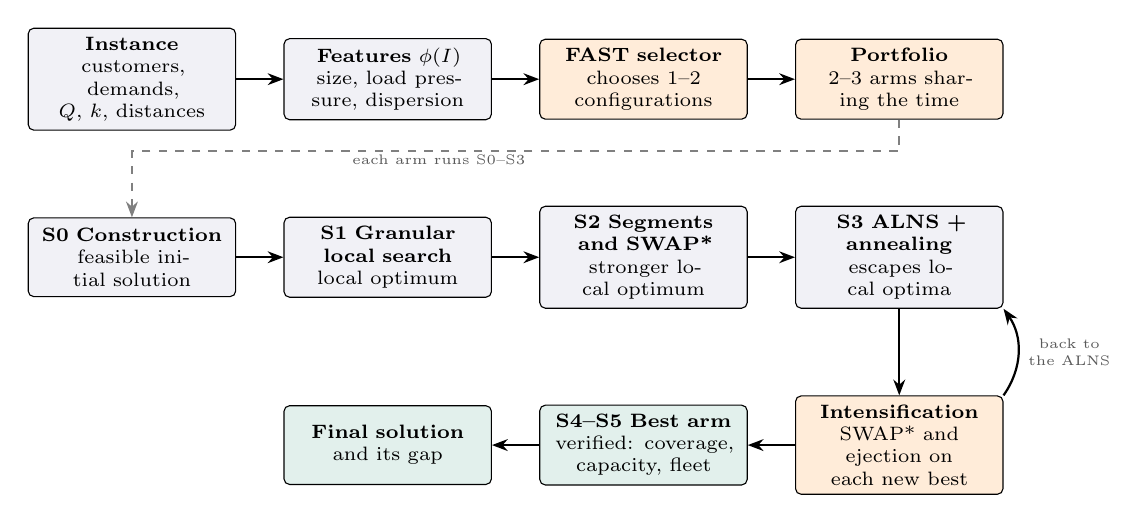
\begin{tikzpicture}[node distance=5mm and 6mm,
  b/.style={draw,rounded corners=2pt,fill=MidnightBlue!6,align=center,font=\scriptsize,minimum height=10mm,text width=24mm},
  o/.style={draw,rounded corners=2pt,fill=orange!15,align=center,font=\scriptsize,minimum height=10mm,text width=24mm},
  g/.style={draw,rounded corners=2pt,fill=sendagreen!12,align=center,font=\scriptsize,minimum height=10mm,text width=24mm},
  f/.style={-{Stealth[length=2mm]},thick},
  lab/.style={font=\tiny,text=gray!70!black,align=center}]
\node[b] (inst) {\textbf{Instance}\\customers, demands,\\$Q$, $k$, distances};
\node[b,right=of inst] (feat) {\textbf{Features $\phi(I)$}\\size, load pressure, dispersion};
\node[o,right=of feat] (sel) {\textbf{FAST selector}\\chooses 1--2 configurations};
\node[o,right=of sel] (arms) {\textbf{Portfolio}\\2--3 arms sharing the time};
\draw[f] (inst)--(feat); \draw[f] (feat)--(sel); \draw[f] (sel)--(arms);
\node[b,below=11mm of inst] (cons) {\textbf{S0 Construction}\\feasible initial solution};
\node[b,right=of cons] (ls) {\textbf{S1 Granular local search}\\local optimum};
\node[b,right=of ls] (seg) {\textbf{S2 Segments and SWAP*}\\stronger local optimum};
\node[b,right=of seg] (alns) {\textbf{S3 ALNS + annealing}\\escapes local optima};
\draw[f] (cons)--(ls); \draw[f] (ls)--(seg); \draw[f] (seg)--(alns);
\draw[f,dashed,gray] (arms.south) -- ++(0,-4mm) -| node[lab,pos=0.3,below,fill=white,inner sep=1pt]{each arm runs S0--S3} (cons.north);
\node[o,below=11mm of alns] (int) {\textbf{Intensification}\\SWAP* and ejection on each new best};
\node[g,left=of int] (best) {\textbf{S4--S5 Best arm}\\verified: coverage, capacity, fleet};
\node[g,left=of best] (out) {\textbf{Final solution}\\and its gap};
\draw[f] (alns)--(int); \draw[f] (int.north east) to[bend right=35] node[lab,right]{back to\\the ALNS} (alns.south east);
\draw[f] (int)--(best); \draw[f] (best)--(out);
\end{tikzpicture}
\caption{Flow of information in \senda. The features of the instance decide how many arms run and with
which configuration. Each arm goes through the chain S0--S3 with its share of the clock;
intensification fires every time the ALNS finds a new global best. At the end each arm is verified
and the best one is kept.}
\label{fig:flujo}
\end{figure}

The order is not arbitrary. Each stage fixes a kind of defect that the previous one cannot see:

\begin{enumerate}[leftmargin=1.5em]
\item \textbf{Construction} quickly produces feasible routes, but with obvious crossings and detours.
\item \textbf{Granular local search} removes those defects with small moves until no small change
improves: the solution sits at a \emph{local optimum}.
\item \textbf{Segments and SWAP*} widen what counts as a ``small move'' and allow escaping local
optima that the basic moves cannot break.
\item The \textbf{ALNS} destroys and rebuilds large parts of the solution, which lets it change its
structure: which customers share a route. That is how it escapes deep local optima.
\item \textbf{Intensification} thoroughly polishes each new best solution.
\item The \textbf{portfolio arms} repeat the process with different configurations and keep the best
result, which reduces the risk of a single trajectory stagnating.
\end{enumerate}

% =========================================================================
\section{The components in detail}
\label{sec:componentes}

Each component is presented with the same questions: what it is, how it works, an example, why it
matters and how much it contributes. The contribution figures come from the ablation of
Section~\ref{sec:ablacion} (what is lost when it is removed) and from the cascade of
Section~\ref{sec:cascada} (what is gained when it is added).

\subsection{Initial construction}
\label{sec:construccion}

\paragraph{What it is.} A fast procedure that produces a first complete solution.

\paragraph{How it works.} If the fleet is fixed, \emph{best-fit-decreasing} (BFD) is used: customers
are sorted from largest to smallest demand and each one is assigned to the vehicle that, after
loading it, would have the least free space left. If it fits in no vehicle, it is assigned to the
least loaded one and the solution is temporarily infeasible; later stages repair it. Within each
vehicle, the customer is inserted at the position that lengthens the route the least. If the fleet
is free, \emph{nearest neighbor} is used: from the depot, the closest customer that still fits is
visited and, when the vehicle is full, a new route is opened.

\begin{ejemplo}[: best-fit-decreasing]
Let $Q=10$, $k=2$ and demands $7,5,4,3,1$. The customer with demand 7 goes to vehicle A (3 left
free). The one with 5 does not fit in A and goes to B (5 left). The one with 4 fits only in B (1
left). The one with 3 fits in A, which becomes full, and the one with 1 fits in B, which becomes
full. Result: A = \{7, 3\} and B = \{5, 4, 1\}, both with load 10.
\end{ejemplo}

\paragraph{Why it matters.} With a fixed fleet, the first thing is to split the demand among the $k$
vehicles without exceeding their capacity, and in many A/B/E instances the total demand almost fills
the fleet. Placing the large customers first, while there is still room, increases the probability
of a feasible split. Construction does not try to make routes short: the following stages take care
of that.

\paragraph{How much it contributes.} It is the starting point (stage S0 of the cascade): on average it
leaves a gap of \cgABEa\,\% on A/B/E and \cgXa\,\% on X.

\subsection{Granular local search}
\label{sec:granular}

\paragraph{What it is.} A procedure that tries small changes to the solution and applies those that
reduce the distance, until none improves it.

\paragraph{How it works.} Five families of moves are used: \emph{relocate} (move a customer to another
position), \emph{swap} (exchange two customers), \emph{2-opt} (reverse a stretch of a route to remove
a crossing), \emph{2-opt*} (exchange the tails of two routes) and \emph{ejection chains} (move a
customer that in turn displaces another). Trying all pairs of customers costs $O(n^2)$ per pass, so
the \emph{granular restriction} of Toth and Vigo~\cite{toth2003granular} is applied: each customer
only considers its $k=15$ nearest neighbors, because it is almost never worth joining two very
distant customers in one route. In addition, each move is evaluated with a constant-time cost
formula, without rebuilding the route. To move customer $u$, whose neighbors in its route are $p_u$
and $n_u$, between nodes $x$ and $y$ of another route:
\begin{equation}
\Delta = \underbrace{d(x,u)+d(u,y)-d(x,y)}_{\text{cost of inserting it}}\;-\;
\underbrace{\bigl[d(p_u,u)+d(u,n_u)-d(p_u,n_u)\bigr]}_{\text{saving from removing it}}.
\label{eq:relocate}
\end{equation}
If $\Delta<0$ and the target route has capacity, the move is applied.

\begin{ejemplo}[: the delta of a relocate]
Let $d(p_u,u)=4$, $d(u,n_u)=5$, $d(p_u,n_u)=7$, $d(x,u)=3$, $d(u,y)=2$ and $d(x,y)=4$. Removing $u$
saves $4+5-7=2$ and inserting it between $x$ and $y$ costs $3+2-4=1$. So $\Delta=1-2=-1$: the move
shortens the solution by one unit. The calculation needed six lookups in the distance matrix,
without traversing any route.
\end{ejemplo}

\paragraph{Why it matters.} It is the tool that does the fine work and the one that runs most often:
stage S1, every ALNS candidate and intensification use it. The granular restriction and constant-time
evaluation let it review many more moves in the same time than a search over all pairs of
customers.

\paragraph{Capacity during polishing.} The initial polish works with a \emph{penalized} cost,
$C(S)+\lambda\cdot\text{excess}(S)$: it tolerates capacity excesses if they save enough distance. If
some excess remains at the end, it repeats the search with a penalty ten times larger to recover
feasibility. That second search does not always succeed: when the load is very tight, the polish may
end with a small excess (Section~\ref{sec:cascada}), and feasibility is recovered later, inside the
ALNS.

\paragraph{How much it contributes.} Removing the granular restriction ---that is, using the full
neighborhood--- worsens the gap on X by 0.267\pp{}: with the same clock, the full neighborhood
evaluates fewer useful iterations.

\subsection{ALNS with simulated annealing}
\label{sec:alns}

\paragraph{What it is.} ALNS (\emph{Adaptive Large Neighborhood Search}~\cite{shaw1998,ropke2006}) is
the main engine. In each iteration it \emph{destroys} part of the solution ---it removes between 10
and 35\,\% of the customers--- and \emph{repairs} it by reinserting them.

\paragraph{Why it is needed.} Local search stops at a local optimum: no small modification improves.
But the best solution may require a large change, for example ten customers changing route at once.
The ALNS causes those large changes in a controlled way.

\paragraph{How it destroys.} There are four operators, each with a different intuition:
\begin{itemize}[leftmargin=1.5em]
\item \emph{random}: removes customers at random to diversify;
\item \emph{worst contribution}: removes, with a random bias, the customers that lengthen their route
the most, that is, those that are probably badly placed;
\item \emph{Shaw}~\cite{shaw1998}: removes a group of customers close to one another, so that they
are redistributed together;
\item \emph{route removal}: removes whole routes. It is the operator meant to reduce the number of
routes; that is why, when the solution exceeds the fleet, it is chosen with probability 0.8.
\end{itemize}

\paragraph{How it repairs.} \emph{Greedy} repair inserts each customer at its cheapest position.
\emph{Regret-2} repair first inserts the customer that would lose the most if left for later.

\begin{ejemplo}[: regret-2 repair]
Customers $a$ and $b$ remain to be inserted. The best insertion of $a$ costs 5 and the second best
12, so its ``regret'' is $12-5=7$. The best for $b$ costs 3 and the second 4: regret 1. Although $b$
is cheaper, regret-2 inserts $a$ first: if another customer takes its best place, $a$ would have to
pay 12, while $b$ would only lose one unit.
\end{ejemplo}

\paragraph{Capacity during repair.} In the standard arms, repair assigns a huge penalty ($10^9$) to
any capacity excess, so in practice it only inserts where the customer fits. The penalized arm of the
portfolio (Section~\ref{sec:portafolio}) relaxes this rule.

\paragraph{How it learns.} Each operator has a weight. It is chosen by roulette, with probability
proportional to its weight, and then updated as $w\leftarrow0.99\,w+0.01\,\sigma$, with reward
$\sigma=5$ if it produced a new global best, 2 if it improved the current solution, 0.5 if it was
only accepted and 0 if it was rejected. This way, operators that work on the current instance are
used more.

\paragraph{How it decides whether to accept.} The repaired candidate is polished with local search
and accepted according to simulated annealing~\cite{kirkpatrick1983}: if it improves, it is always
accepted; if it worsens by $\Delta$, it is accepted with probability $e^{-\Delta/T}$. The temperature
decreases geometrically, $T(f)=T_0(T_f/T_0)^f$, where $f\in[0,1]$ is the fraction of the budget
used, $T_0=0.02\,C$ and $T_f=0.0002\,C$, with $C$ the cost of the best initial solution.

\begin{ejemplo}[: accepting a worse solution]
If the candidate is 10 units longer ($\Delta=10$) and the temperature is $T=20$, it is accepted with
probability $e^{-10/20}=0.61$. At the end of the search, with $T=1$, the same decision would have
probability $e^{-10}\approx0.00005$. The algorithm explores a lot at the beginning and becomes
demanding at the end.
\end{ejemplo}

\begin{algorithm}[H]
\caption{ALNS core of one \senda{} arm}
\label{alg:alns}
\begin{algorithmic}[1]
\Require solution $S$ (already polished), budget $B$ in seconds or iterations
\Ensure best feasible solution $S^\star$
\State $S^\star\gets S$; weights $w\gets\mathbf{1}$
\While{$B$ is not exhausted and there have not been 5\,000 consecutive iterations without improvement}
  \State choose destroy $\delta$ and repair $\rho$ by roulette with weights $w$
  \State $S'\gets\rho(\delta(S))$; polish $S'$ with granular local search
  \If{$S'$ is feasible and $C(S')<C(S^\star)$}
     \State intensify $S'$ (SWAP* and ejection); $S^\star\gets S'$; $S\gets S'$; $\sigma\gets5$
  \ElsIf{$\Delta=C(S')-C(S)<0$ or $u\sim U(0,1)<e^{-\Delta/T(f)}$}
     \State $S\gets S'$; $\sigma\gets 2$ if $\Delta<0$, otherwise $0.5$
  \Else
     \State $\sigma\gets0$
  \EndIf
  \State $w_\delta\gets0.99\,w_\delta+0.01\,\sigma$; \ $w_\rho\gets0.99\,w_\rho+0.01\,\sigma$
\EndWhile
\State \Return $S^\star$
\end{algorithmic}
\end{algorithm}

\paragraph{Why it matters and how much it contributes.} It is the dominant component. In the ablation,
removing the ALNS ---leaving only construction and polishing--- raises the mean gap on X from
4.285\,\% to 16.702\,\%: a loss of 12.4 points. In the cascade (Section~\ref{sec:cascada}), the ALNS
is the first stage that always delivers feasible solutions, and on A/B/E it lowers the gap of the
feasible solutions from \cgfABEc\,\% to \cgfABEd\,\%.

\subsection{Segment moves and Or-opt-3}
\label{sec:segmentos}

\paragraph{What it is.} An extension of local search: instead of moving one customer, a
\emph{segment} of two or three consecutive customers is moved (\emph{relocate-2}, \emph{Or-opt-3}),
or a pair of customers is exchanged for a single one (\emph{swap-2}).

\paragraph{Why it matters.} Often two consecutive customers are well placed next to each other, but
the whole pair would be better in another route. Moving them separately takes two steps, and the
first one almost always worsens the solution, so local search does not take it. Moving them together
turns that improvement into a single step that is detected.

\paragraph{How much it contributes.} Removing them raises the gap on X by 0.528\pp{}; on 36 of 41
instances the full version is better. It is the second most important component after the ALNS.

\subsection{SWAP*}
\label{sec:swapstar}

\paragraph{What it is.} A move between two routes proposed by Vidal for
HGS-CVRP~\cite{vidal2022hgs}. The classic \emph{swap} exchanges customer $u$ of route A with customer
$v$ of route B, and each takes the exact position of the other. SWAP* also exchanges them, but places
each one at its \emph{best} position in the other route.

\begin{figure}[H]
\centering
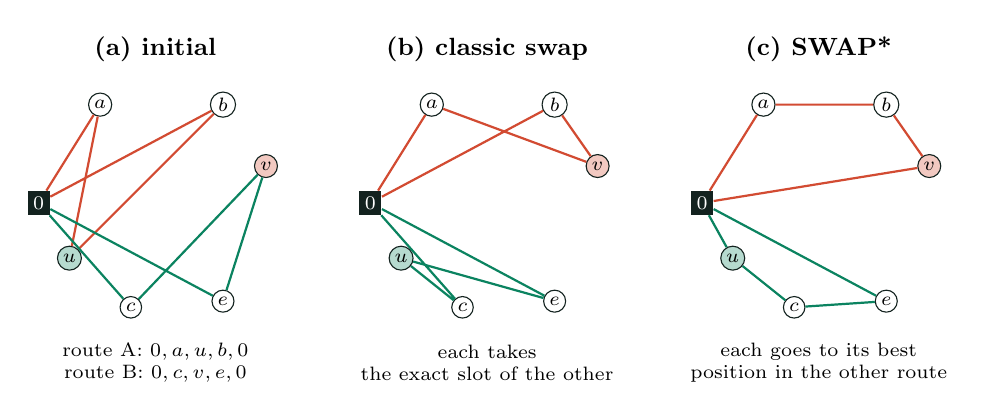
\begin{tikzpicture}[scale=0.78,
  n/.style={circle,draw=sendaink,fill=white,inner sep=1.1pt,font=\scriptsize},
  d/.style={rectangle,fill=sendaink,text=white,inner sep=2pt,font=\scriptsize}]
% Fixed positions of the points (the same in the three panels).
\newcommand{\puntos}{%
  \node[d] (nD) at (0,0) {0};
  \node[n] (nA) at (1,1.6) {$a$}; \node[n] (nB) at (3,1.6) {$b$};
  \node[n,fill=sendagreen!30] (nU) at (0.5,-0.9) {$u$}; \node[n,fill=sendared!30] (nV) at (3.7,0.6) {$v$};
  \node[n] (nC) at (1.5,-1.7) {$c$}; \node[n] (nE) at (3,-1.6) {$e$};}
\begin{scope}
\puntos
\node[font=\small\bfseries] at (1.9,2.5) {(a) initial};
\draw[thick,sendared] (nD)--(nA)--(nU)--(nB)--(nD);
\draw[thick,sendagreen] (nD)--(nC)--(nV)--(nE)--(nD);
\node[font=\scriptsize,align=center] at (1.9,-2.6) {route A: $0,a,u,b,0$\\route B: $0,c,v,e,0$};
\end{scope}
\begin{scope}[xshift=5.4cm]
\puntos
\node[font=\small\bfseries] at (1.9,2.5) {(b) classic swap};
\draw[thick,sendared] (nD)--(nA)--(nV)--(nB)--(nD);
\draw[thick,sendagreen] (nD)--(nC)--(nU)--(nE)--(nD);
\node[font=\scriptsize,align=center] at (1.9,-2.6) {each takes\\the exact slot of the other};
\end{scope}
\begin{scope}[xshift=10.8cm]
\puntos
\node[font=\small\bfseries] at (1.9,2.5) {(c) SWAP*};
\draw[thick,sendared] (nD)--(nA)--(nB)--(nV)--(nD);
\draw[thick,sendagreen] (nD)--(nU)--(nC)--(nE)--(nD);
\node[font=\scriptsize,align=center] at (1.9,-2.6) {each goes to its best\\position in the other route};
\end{scope}
\end{tikzpicture}
\caption{Difference between the classic swap and SWAP*. The points do not move; only the routes
change. In (a), $u$ is badly placed in the red route and $v$ in the green one. The classic swap (b)
exchanges them, but each ends up in the slot the other left, far from where it should be. SWAP* (c)
exchanges them and places each at its best position, so it finds improvements that the classic swap
discards.}
\label{fig:swapstar}
\end{figure}

\paragraph{How it works.} The cost change is
\begin{equation}
\Delta_{\mathrm{SWAP^{*}}}(u,v) \;=\; \mathrm{ins}^{*}_{B\setminus v}(u)+\mathrm{ins}^{*}_{A\setminus u}(v)
\;-\;\mathrm{rem}_{A}(u)-\mathrm{rem}_{B}(v),
\label{eq:swapstar}
\end{equation}
where $\mathrm{rem}$ is what is saved by removing the customer from its route and $\mathrm{ins}^*$
the cost of its best insertion in the other route. To make it fast, the three best insertion
positions of each customer in each route are stored in advance; this way, the best place is obtained
in constant time even if the outgoing customer occupies one of them. The original version chooses
which pairs of routes to compare using polar sectors, which requires coordinates; ours uses the
granular graph and also works with distance matrices without coordinates.

\begin{ejemplo}[: why SWAP* finds more]
Removing $u$ from A saves 10 and removing $v$ from B saves 9. In the classic swap, $u$ in the slot of
$v$ costs 12 and $v$ in the slot of $u$ costs 11: $\Delta=12+11-10-9=+4$, so it is rejected. In
SWAP*, the best position of $u$ in B costs 7 and that of $v$ in A costs 8: $\Delta=7+8-10-9=-4$, and
the exchange improves the solution by 4 units.
\end{ejemplo}

\paragraph{Why it matters and how much it contributes.} It explores much richer exchanges between
routes at the same cost per evaluation. Removing it raises the gap on X by 0.413\pp{}, with 38 of 41
instances in favor of the full version. It is applied in the initial polish and in intensification,
but not to every ALNS candidate, because that would reduce the number of iterations too much.

\subsection{Intensification of the global best}
Every time the ALNS finds a new best feasible solution, it is polished thoroughly: granular local
search, up to two passes of SWAP* and ejection chains, with a maximum of 50 polishes per arm. This is
when SWAP* and ejection chains do their work: they are reserved for solutions that have already
proven promising.

\subsection{FAST selector}
\label{sec:fast}

\paragraph{What it is.} A frozen rule that, from features that are cheap to compute, decides which
additional configuration to run besides the base one.

\paragraph{How it works.} It computes the number of customers $n$, the fleet $k$, the load pressure
$\sum q_i/(kQ)$, the coefficients of variation of the demand and of the distance to the depot, the
angular concentration of the customers around the depot and their density. With those values it
walks a list of conditions (Appendix~\ref{app:selector}) and the first one that holds chooses one of
the configurations in Table~\ref{tab:ramas}: wider neighborhoods, more aggressive destruction or more
iterations.

\begin{table}[H]
\centering
\caption{Configurations the selector can choose. All use segments and SWAP* with two passes.}
\label{tab:ramas}
\small
\begin{tabular}{@{}llcc@{}}
\toprule
Configuration & Idea & neighbors $k$ & destruction \\
\midrule
\tsl{baseline\_cap2\_calls50} & base branch, always runs & 15 & 10--35\,\% \\
\tsl{granular\_k25} / \tsl{granular\_k40} & wider neighborhood & 25 / 40 & 10--35\,\% \\
\tsl{large\_destroy\_k25} & more aggressive destruction & 25 & 15--45\,\% \\
\tsl{medium\_destroy\_k25} & moderate destruction & 25 & 10--25\,\% \\
\tsl{long\_10k\_k25} & up to 10\,000 iterations & 25 & 10--35\,\% \\
\bottomrule
\end{tabular}
\end{table}

\paragraph{Why it matters and how much it contributes.} There is no ideal configuration for every
instance: with very variable demand it pays to destroy more; with concentrated customers, to widen
the neighborhood. Replacing the chosen branch with a restart of the base branch raises the gap on X
by 0.145\pp{}.

\subsection{The portfolio: the evaluated configuration}
\label{sec:portafolio}

\paragraph{What it is.} It is the frozen configuration of SENDA evaluated on A/B/E. Its operational
definition:
\begin{enumerate}[leftmargin=1.5em]
\item one arm with the base configuration and another with the configuration chosen by FAST, if
different;
\item Or-opt-3 active and a stagnation cut: an arm stops after 5\,000 iterations without improvement;
\item an additional \textbf{penalized arm} with the last configuration.
\end{enumerate}
Each arm receives an equal share of the clock (80\,\% of the budget divided among 2 or 3 arms) and the
best verified result is kept. On X the FAST-PEN4 variant was used, which differs in that its standard
arms use neither Or-opt-3 nor the stagnation cut.

\paragraph{The penalized arm.} In the standard arms, the ALNS repair treats capacity as a hard
constraint: it never accepts an excess. The penalized arm allows passing through solutions with
capacity excess, paying a proportional penalty:
\begin{equation}
C_\lambda(S)=C(S)+\lambda\cdot\sum_{r\in S}\max\Bigl(0,\;\sum_{i\in r}q_i-Q\Bigr).
\end{equation}
The weight $\lambda$ adjusts automatically every 50 iterations: if fewer than 25\,\% of the candidates
are feasible, $\lambda$ grows by 25\,\%; if more than 45\,\% are, it decreases by 15\,\%. This keeps
the search near the frontier between feasible and infeasible solutions, which is where the best ones
usually are.

\begin{ideaclave}[: why penalization helps]
When capacity is very tight, the feasible solutions form separate islands: to go from a good one to
a better one you have to cross solutions with excess. The penalty builds that bridge. Since only the
best \emph{feasible} solution of each arm counts, the penalized arm never delivers an invalid
solution. Its cost is something else: it uses its share of the clock, which in the worst case
contributes nothing.
\end{ideaclave}

\paragraph{How much it contributes.} Replacing the penalized arm with a normal restart of the same
time raises the gap on X by 0.145\pp{} (23 instances in favor and 18 against; $p_H=0.048$, the weakest
evidence of the ablation). In a comparison at equal computation, adding it reduces the gap on X from
3.678\,\% to 3.461\,\% (31 of 41 instances, $p=4.3\times10^{-5}$).

\subsection{Parameters}
\begin{table}[H]
\centering
\caption{Solver parameters. None is tuned per instance.}
\label{tab:parametros}
\small
\begin{tabular}{@{}lll@{}}
\toprule
Component & Parameter & Value \\
\midrule
Granular & neighbors per customer (all if $n\le60$) & 15 \\
ALNS & destroyed fraction & $U(0.10,0.35)$ depending on branch \\
ALNS & weight decay; rewards & 0.99; 5 / 2 / 0.5 / 0 \\
Annealing & $T_0$, $T_f$ (fraction of the cost) & 0.02, 0.0002 \\
Fleet & probability of forcing route removal & 0.8 \\
Intensification & SWAP* passes; polishes per arm & 2; 50 \\
Portfolio & stagnation cut; clock reserve & 5\,000 iterations; 20\,\% \\
Penalized arm & $\lambda$ adjustment every 50 iterations & $\times1.25$ / $\times0.85$ \\
\bottomrule
\end{tabular}
\end{table}

% =========================================================================
\section{How quality accumulates: the cascade experiment}
\label{sec:cascada}

The ablation answers ``how much is lost if I remove a component?''. The cascade answers the
complementary question: ``what quality do I have after each stage?''. Six stages were run with the
same 10 seeds of the protocol, on the 63 A/B/E instances (fixed fleet) and the 41 X instances (free
fleet). The component-ablation binary was used, because it is the only one that allows stopping the
solver before the ALNS; its full version obtained a gap of 4.285\,\% on X, close to but not identical
to the 4.119\,\% of the confirmatory binary. The stages are:

\begin{center}
\small
\begin{tabular}{@{}ll@{}}
\toprule
Stage & Solution available \\
\midrule
S0 & construction, with no improvement \\
S1 & construction + basic granular local search \\
S2 & construction + local search with segments, Or-opt-3 and SWAP* \\
S3 & first arm of the full portfolio (with ALNS), with its share of the clock \\
S4 & best of S3 and the arm with the configuration chosen by FAST \\
S5 & full portfolio: the penalized arm is added \\
\bottomrule
\end{tabular}
\end{center}

\noindent S1 and S2 are two independent polishes of the same construction: S2 does not start from S1,
but uses a richer set of moves. That is why, in a particular replicate, S2 may end up worse than S1,
even though it is better on average. Likewise, each arm of S3--S5 does its own construction, polish
and ALNS.

Three measures are reported for each stage, because a single one is misleading:
\begin{itemize}[leftmargin=1.5em]
\item the \textbf{percentage of feasible solutions} the stage delivers;
\item the \textbf{gap of the feasible solutions}, averaged first per instance (in parentheses, how
many instances had at least one feasible replicate);
\item the \textbf{available gap}, the rule fixed before seeing the results: if the stage delivers an
infeasible solution, the solution actually in hand is still the construction.
\end{itemize}

\begin{table}[H]
\centering
\caption{Quality after each stage (10 replicates per instance). ``Feas.'' is the percentage of
feasible solutions; ``feasible gap'' averages only the feasible solutions (in parentheses, the number
of instances with at least one); ``available gap'' replaces each infeasible solution with the
construction.}
\label{tab:cascada}
\footnotesize
\setlength{\tabcolsep}{3.5pt}
\begin{tabular}{@{}lrrrcrrr@{}}
\toprule
 & \multicolumn{3}{c}{A/B/E (63 inst., 2\,s, fixed fleet)} & & \multicolumn{3}{c}{X (41 inst., 4\,s)} \\
\cmidrule{2-4}\cmidrule{6-8}
Stage & feas. & feasible gap & available gap & & feas. & feasible gap & available gap \\
\midrule
S0 construction & \cfeABEa\,\% & \cgfABEa\,\% (\cnfABEa) & \cgABEa\,\% & & \cfeXa\,\% & \cgfXa\,\% (\cnfXa) & \cgXa\,\% \\
S1 + granular local & \cfeABEb\,\% & \cgfABEb\,\% (\cnfABEb) & \cgABEb\,\% & & \cfeXb\,\% & \cgfXb\,\% (\cnfXb) & \cgXb\,\% \\
S2 + segments and SWAP* & \cfeABEc\,\% & \cgfABEc\,\% (\cnfABEc) & \cgABEc\,\% & & \cfeXc\,\% & \cgfXc\,\% (\cnfXc) & \cgXc\,\% \\
S3 + ALNS (base arm) & \cfeABEd\,\% & \cgfABEd\,\% (\cnfABEd) & \cgABEd\,\% & & \cfeXd\,\% & \cgfXd\,\% (\cnfXd) & \cgXd\,\% \\
S4 + FAST branch & \cfeABEe\,\% & \cgfABEe\,\% (\cnfABEe) & \cgABEe\,\% & & \cfeXe\,\% & \cgfXe\,\% (\cnfXe) & \cgXe\,\% \\
S5 + penalized arm & \cfeABEf\,\% & \cgfABEf\,\% (\cnfABEf) & \cgABEf\,\% & & \cfeXf\,\% & \cgfXf\,\% (\cnfXf) & \cgXf\,\% \\
\bottomrule
\end{tabular}
\end{table}

\begin{figure}[H]
\centering
\begin{tikzpicture}
\begin{axis}[ybar,width=0.48\linewidth,height=5.4cm,ymode=log,ymin=0.05,ymax=200,title={A/B/E},title style={font=\small},
  symbolic x coords={S0,S1,S2,S3,S4,S5},xtick=data,ylabel={gap of feasible solutions (\%)},bar width=11pt,
  nodes near coords,nodes near coords style={font=\tiny},point meta=rawy,
  every node near coord/.append style={/pgf/number format/fixed,/pgf/number format/precision=2},
  tick label style={font=\scriptsize},label style={font=\small},enlarge x limits=0.12,log origin=infty]
\addplot[fill=sendared!70,draw=sendared] table[x=etapa,y=abe_f]{datos/cascada.dat};
\end{axis}
\end{tikzpicture}\hfill
\begin{tikzpicture}
\begin{axis}[ybar,width=0.48\linewidth,height=5.4cm,ymode=log,ymin=1,ymax=60,title={X},title style={font=\small},
  symbolic x coords={S0,S1,S2,S3,S4,S5},xtick=data,bar width=11pt,
  nodes near coords,nodes near coords style={font=\tiny},point meta=rawy,
  every node near coord/.append style={/pgf/number format/fixed,/pgf/number format/precision=2},
  tick label style={font=\scriptsize},label style={font=\small},enlarge x limits=0.12,log origin=infty]
\addplot[fill=MidnightBlue!60,draw=MidnightBlue] table[x=etapa,y=x_f]{datos/cascada.dat};
\end{axis}
\end{tikzpicture}
\caption{Gap of the feasible solutions after each stage (logarithmic scale). On A/B/E the decisive drop
happens when the ALNS comes in (S3); on X local search already does much of the work and the extra
arms (S4, S5) contribute more than on A/B/E.}
\label{fig:cascada}
\end{figure}

\begin{ejemplo}[: a solution in transit]
On instance \tsl{\trazaInst} (BKS \trazaBKS), replicate 0, the cost evolves like this: construction
\trazaA; local search \trazaB; segments and SWAP* \trazaC; first arm with ALNS \trazaD; with the FAST
branch \trazaE; and with the penalized arm \trazaF.
\end{ejemplo}

\paragraph{Reading.}
\begin{enumerate}[leftmargin=1.5em]
\item \textbf{Construction does not look for short routes.} Best-fit-decreasing splits the demand
without looking at geography, which is why on A/B/E it leaves gaps close to 80\,\%. On X, nearest
neighbor does look at distances and starts from a smaller gap.
\item \textbf{Local search makes the largest reduction in distance.} With the polish alone, the gap of
the feasible solutions drops to \cgfABEb\,\% on A/B/E and to \cgfXb\,\% on X.
\item \textbf{Segments and SWAP* shorten further, but break capacity.} The feasible solutions of S2 are
better than those of S1, but only \cfeABEc\,\% of the S2 polishes ended feasible on A/B/E
(\cfeXc\,\% on X). The penalized polish crosses into the infeasible region to save distance and does
not always manage to come back. That is why the available gap of S2 is bad: in half of the cases
there is nothing but the construction.
\item \textbf{The ALNS is the first stage that delivers both quality and feasibility in 100\,\% of the
trials.} On A/B/E it lowers the gap to \cgABEd\,\%, with a median close to zero. Its repair and its
local search treat capacity as a hard constraint at every iteration.
\item \textbf{The extra arms fine-tune.} On A/B/E, the FAST branch and the penalized arm reduce the gap
from \cgABEd\,\% to \cgABEf\,\%, and the number of instances that reach the BKS in all their
replicates goes from \cbABEd{} to \cbABEf{}. On X, where a single arm has little time, their relative
contribution is larger: from \cgXd\,\% to \cgXf\,\%.
\end{enumerate}

\begin{leccion}[: an invalid solution always looks better]
If the cost of all S2 solutions were averaged, including the infeasible ones, its gap would be
\cgrABEc\,\% on A/B/E: \emph{better} than that of the ALNS (\cgABEd\,\%). It is the same trap as the
case study of Section~\ref{sec:caso}: violating a constraint ---capacity or fleet--- almost always
allows shorter routes. That is why every comparison must count only verified solutions.
\end{leccion}

\begin{leccion}[: cascade and ablation do not say the same thing]
In the cascade, what is attributed to each stage depends on the order in which they are added: local
search seems to do most of the work because it goes first and finds a solution with plenty of room
for improvement. In the ablation, removing a component measures what the others \emph{cannot}
compensate: without the ALNS, the gap on X rises 12.4 points, because local search alone does not
reach the solutions the ALNS does find. Both views are needed. For example, the cascade does not show
the value of the granular restriction, because it is not a stage but the way all of them run; only
the ablation reveals it.
\end{leccion}

% =========================================================================
\section{Computational complexity: how much each step costs}
\label{sec:complejidad}

The previous sections explained what each component does and how much quality it contributes. An
equally important question remains: \emph{how much does it cost}. In SENDA the budget is a fixed
clock, so the cost of each step decides how many iterations fit in that clock and, with that, how far
the search gets. This section introduces the tool to reason about that cost, big-$O$ notation,
applies it to each component and checks the prediction with a measurement.

\subsection{Big-$O$ notation}

Counting seconds does not work for comparing algorithms: the same program takes a different time on
each computer. What is stable is \emph{how} the number of operations \emph{grows} when the input size
$n$ grows. Big-$O$ notation describes that growth. An algorithm is said to be $O(g(n))$ if, beyond a
certain size, its number of operations never exceeds a fixed multiple of $g(n)$. Formally,
$f(n)=O(g(n))$ if there exist constants $c>0$ and $n_0$ such that
\begin{equation}
f(n)\;\le\;c\cdot g(n)\qquad\text{for all } n\ge n_0 .
\end{equation}
In practice three rules are enough:
\begin{itemize}[leftmargin=1.5em]
\item \textbf{Constants and lower-order terms are dropped.} $3n^2+50n+7$ is $O(n^2)$: for large $n$,
the $n^2$ term dominates the others.
\item \textbf{Steps in sequence add up and the largest dominates.} Sorting ($O(n\log n)$) and then
walking the list ($O(n)$) costs $O(n\log n)$.
\item \textbf{Nested loops multiply.} Visiting each customer and, for each one, all the others costs
$O(n\cdot n)=O(n^2)$.
\end{itemize}

\begin{table}[H]
\centering
\caption{How the most common complexity functions grow. Logarithms are base 2.}
\label{tab:crecimiento}
\small
\begin{tabular}{@{}lrrl@{}}
\toprule
Function & $n=100$ & $n=1\,000$ & Example in this guide \\
\midrule
$O(1)$        & 1 & 1 & evaluating the delta of a move (Eq.~\ref{eq:relocate}) \\
$O(\log n)$   & 6.6 & 10 & --- \\
$O(n)$        & 100 & 1\,000 & computing the cost of a solution \\
$O(n\log n)$  & 664 & 9\,966 & sorting customers by demand \\
$O(n^2)$      & $10^4$ & $10^6$ & computing the distance matrix \\
$O(n^3)$      & $10^6$ & $10^9$ & regret-2 repair with fixed-length routes \\
$O(2^n)$      & $1.3\times10^{30}$ & $1.1\times10^{301}$ & trying every subset of customers \\
$O(n!)$       & $9.3\times10^{157}$ & $4.0\times10^{2567}$ & trying every visiting order \\
\bottomrule
\end{tabular}
\end{table}

\begin{ideaclave}[: big-$O$ describes growth, not time]
Two $O(n)$ algorithms can take very different times: the notation hides the constants. What it does
say is what happens as the instance grows. If a step is $O(n^2)$, doubling the number of customers
multiplies its cost by about 4; if it is $O(n^3)$, by about 8.
\end{ideaclave}

\subsection{Why the CVRP is not solved exactly}

The CVRP is \emph{NP-hard}~\cite{lenstra1981}: it contains the traveling salesman problem as a special
case (a single vehicle with enough capacity), and no algorithm is known that solves it exactly in
polynomial time, that is, in $O(n^c)$ for some constant $c$. An exhaustive search would have to
review, just for the visiting order, on the order of $n!$ possibilities, plus every way of splitting
the customers among vehicles.

\begin{ejemplo}[: the size of the search space]
With a single vehicle and $n=20$ customers there are $20!\approx2.4\times10^{18}$ visiting orders. A
computer that evaluated one billion orders per second would need
$2.4\times10^{18}/10^9\approx2.4\times10^{9}$ seconds: about 77 years. With 21 customers, 21 times
longer.
\end{ejemplo}

Modern exact methods certify optima on many reference instances~\cite{queiroga2021}, but their time
grows in ways that are hard to predict. A heuristic trades the guarantee of optimality for something
that can be controlled: each iteration costs a \emph{polynomial} number of operations, and the number
of iterations is set by the clock.

\subsection{Notation for the analysis}

Besides $n$ (number of customers), the cost of SENDA depends on four quantities:
\begin{itemize}[leftmargin=1.5em]
\item $k$: neighbors per customer in the granular restriction (15, 25 or 40 depending on the branch;
all other customers if $n\le60$);
\item $R$: number of routes;
\item $L\approx n/R$: average length of a route, in customers;
\item $q$: customers removed by an ALNS destruction, $q=\theta n$ with $\theta$ between 0.10 and 0.35
(Table~\ref{tab:parametros}).
\end{itemize}
Routes are stored as arrays of customers. Inserting or removing a customer from an array requires
shifting the ones that follow it, so it costs $O(L)$.

\subsection{Cost of each component}

Table~\ref{tab:complejidad} summarizes the analysis of the code in \tsl{native/senda\_core.cpp}. The
figures are worst case per call.

\begin{table}[htbp]
\centering
\caption{Complexity of each SENDA component.}
\label{tab:complejidad}
\footnotesize
\begin{tabular}{@{}>{\raggedright\arraybackslash}p{4.3cm}>{\raggedright\arraybackslash}p{4.4cm}>{\raggedright\arraybackslash}p{6.5cm}@{}}
\toprule
Component & Cost & Where it comes from \\
\midrule
\multicolumn{3}{@{}l}{\emph{Once per run}} \\
Distance matrix & $O(n^2)$ & one distance per pair of nodes; 4 bytes per pair (4\,MB with 1\,000 customers) \\
Granular neighbor lists & $O(n^2\log n)$ & for each customer the distances to the others are sorted \\
\emph{Best-fit-decreasing} construction & $O(n\log n+nR+nL)$ & sort; choose a vehicle; insert at the best position \\
Nearest-neighbor construction & $O(n^2)$ & at each step the closest customer among those left is searched \\
\midrule
\multicolumn{3}{@{}l}{\emph{Local search}} \\
Evaluating a move & $O(1)$ & six to eight lookups in the matrix (Eq.~\ref{eq:relocate}) \\
Applying a move & $O(L)$ & insert or remove in the route array and update its loads \\
One granular pass & $O(nk)$ evaluations & each customer tries its $k$ neighbors with each family of moves \\
\midrule
\multicolumn{3}{@{}l}{\emph{One ALNS iteration}} \\
Random destruction & $O(n)$ & shuffle and remove \\
Worst-contribution destruction & $O(n\log n+qn)$ & sort by contribution; each removal reshuffles the list \\
Shaw destruction & $O(qn\log n)$ & before each removal the list is re-sorted by closeness \\
Route destruction & $O(n+R\log R)$ & choose routes and separate their customers \\
Greedy repair & $O(q(n+k+R))$ & per customer: reindex the solution and review its insertion options \\
Regret-2 repair & $O(qn+q^2(k+R)\log(k+R))$ & each round recomputes and sorts the options of \emph{all} pending customers \\
\midrule
\multicolumn{3}{@{}l}{\emph{Intensification}} \\
SWAP* (one pass) & $O(PL^2)$ & $P\le\min(R^2,nk)$ pairs of neighboring routes; in each pair, the three best insertions of each customer in the other route \\
Ejection chains (one pass) & $O(nRL^3)=O(n^2L^2)$ & each customer against each full route, each pair of customers to eject and one reinsertion per combination \\
Removing a surplus route & $O(n^2)$ & each candidate route reinserts its customers at every position of the others \\
\bottomrule
\end{tabular}
\end{table}

\begin{ejemplo}[: why the granular restriction changes the order of magnitude]
With $n=400$, a pass that tried every pair of customers would make about $400^2=160\,000$ evaluations
per family of moves. With $k=15$ it makes $400\times15=6\,000$: 27 times fewer. Since each evaluation
is $O(1)$, the full pass goes from $O(n^2)$ to $O(nk)$, which is linear in $n$ because $k$ is fixed.
\end{ejemplo}

\paragraph{The cost of one ALNS iteration.} An iteration adds up one destruction, one repair, the local
search of the candidate and the computation of its cost ($O(n)$). Local search has a time cap (0.08\,s
per candidate), so it does not grow without bound. With $q=\theta n$, the dominant terms are the Shaw
destruction, $O(n^2\log n)$, and the regret-2 repair, $O(n^2(k+R)\log(k+R))$. If the route length is
fixed, $R$ grows with $n$ and regret-2 approaches $O(n^3)$. The prediction is, then, that an
iteration becomes between 4 and 8 times more expensive each time $n$ doubles.

\paragraph{Why SWAP* and ejection chains are kept in reserve.} One pass of ejection chains is
$O(n^2L^2)$: with 400 customers in routes of 12 there are on the order of a million combinations
(incoming customer, target route and pair of ejected customers), each with reinsertions of cost
$O(L)$, about $2\times10^{7}$ steps per pass. Applying it to every ALNS candidate would use up the
clock in a few iterations. That is why SWAP* and the chains are only applied in the initial polish
and to each new global best (Section~\ref{sec:swapstar}): they are expensive operators used where
they pay off the most.

\subsection{Experimental check}

To contrast the analysis with the real program, we measured how many ALNS iterations SENDA completes
in a fixed clock, on random instances of 100 to 800 customers. Table~\ref{tab:medicion} and
Figure~\ref{fig:complejidad} show the result.

\begin{table}[H]
\centering
\caption{ALNS iterations in 4\,s (one thread, median of 3 seeds) and mean time per iteration.}
\label{tab:medicion}
\small
\begin{tabular}{@{}rrrr@{}}
\toprule
$n$ & Iterations & ms per iteration & Factor when doubling $n$ \\
\midrule
100 & 11\,073 & 0.32 & --- \\
200 & 2\,714 & 1.30 & $\times$4.1 \\
400 & 703 & 5.01 & $\times$3.9 \\
800 & 99 & 35.56 & $\times$7.1 \\
\bottomrule
\end{tabular}
\end{table}

\begin{figure}[H]
\centering
\begin{tikzpicture}
\begin{loglogaxis}[width=0.8\linewidth,height=6.2cm,xlabel={number of customers $n$},
  ylabel={ms per ALNS iteration},grid=major,grid style={gray!20},
  xtick={100,200,400,800},xticklabels={100,200,400,800},
  legend pos=north west,legend style={font=\scriptsize},tick label style={font=\scriptsize},
  label style={font=\small}]
\addplot[only marks,mark=*,mark size=2.2pt,sendared] table[x=n,y=ms]{datos/complejidad.dat};
\addlegendentry{SENDA (measured)}
\addplot[domain=100:800,samples=20,thick,MidnightBlue] {0.318*(x/100)^2};
\addlegendentry{reference $\propto n^2$}
\addplot[domain=100:800,samples=20,thick,dashed,sendagreen] {0.318*(x/100)^3};
\addlegendentry{reference $\propto n^3$}
\end{loglogaxis}
\end{tikzpicture}
\caption{Time per iteration versus $n$ on a logarithmic scale. On this scale, a function $c\,n^a$ is a
straight line with slope $a$. Up to 400 customers the points follow the $n^2$ reference; from 400 to
800 the slope approaches that of $n^3$.}
\label{fig:complejidad}
\end{figure}

The measurement confirms the analysis. Between 100 and 400 customers, each doubling of $n$ multiplies
the cost of an iteration by about 4, as befits an $O(n^2)$ cost. From 400 to 800 the factor rises to
7.1, closer to $n^3$: this is expected when the $q^2R$ term of regret-2 starts to weigh, although in
that range intensification also plays a role, because each polish of the global best costs more and
there are fewer iterations to spread it over. The measurement does not separate the two effects.

\begin{leccion}[: with a fixed clock, complexity turns into quality]
With a cost per iteration of order $n^2$, the number of iterations that fit in the clock falls as
$1/n^2$: from 100 to 400 customers, from 11\,073 to 703 iterations, 16 times fewer. This is consistent
with what was observed on the X instances (Section~\ref{sec:resultados}): with 199 to 428 customers
and little more than one second per arm, the ALNS has on the order of hundreds of iterations and
barely improves what local search already achieved. For a heuristic to scale it is not enough for
each step to be polynomial; the exponent matters.
\end{leccion}

\begin{reproducir}
Binary compiled from \tsl{native/senda\_core.cpp} (SHA-256 \tsl{d63db4bc6436\ldots}) with
\tsl{python -m lattimex build}; direct call to \tsl{senda\_solve} with a 4\,s clock, free fleet,
$k=15$, segment moves and SWAP* active (\tsl{use\_segment\_moves=3}), no penalized arm and seeds 1, 2
and 3. Instances: depot and customers uniform in $[0,1000]^2$, integer demands uniform between 1 and
10, capacity 66 (about 12 customers per route). Machine: Intel Core i5-8250U. Absolute figures change
with the machine; the factors when doubling $n$ are what should be reproduced.
\end{reproducir}

\subsection{Where the cost could go down}

The analysis also points to possible improvements. None is applied in the engine; they are proposed
as exercises.
\begin{enumerate}[leftmargin=1.5em]
\item \textbf{Shaw destruction without re-sorting.} Instead of sorting the whole list before each
removal ($O(n\log n)$), choose among the granular neighbors of the reference customer, which are
already sorted: $O(k)$ per removal.
\item \textbf{Incremental regret-2.} When a customer is inserted only the options that touch the
modified route change. Keeping the two best options of each pending customer and recomputing only the
affected ones avoids repeating the work for all pending customers in every round.
\item \textbf{Neighbors by partial selection.} To obtain the $k$ nearest it is not necessary to sort
all of them: \tsl{std::nth\_element} separates them in $O(n)$ per customer, and building the lists
drops from $O(n^2\log n)$ to $O(n^2)$.
\end{enumerate}

% =========================================================================
\section{How to evaluate a heuristic without fooling yourself}
\label{sec:evaluar}

A heuristic is random and its quality depends on the time it is given. That is why the way it is
measured matters as much as the algorithm. This project followed six rules.

\paragraph{1. The same clock for everyone.} The main profile gives each trial 2\,s of wall-clock time
on a single thread on A/B/E and 4\,s on X, with a 10\,\% tolerance. A trial that exceeds the
tolerance is discarded. SENDA reserves 20\,\% of the limit for reading the instance and verifying the
solution, so its core uses the remaining 80\,\%.

\paragraph{2. Replicates, not the best of ten.} Each instance is solved 10 times with different seeds
and the \emph{mean} is reported. Choosing the best of ten runs exaggerates the quality a user would
get from a single execution.

\paragraph{3. Independent and uniform verification.} Each solution is checked outside the solver:
coverage, capacity, fleet and cost are recomputed. The rule must be \emph{the same} for all methods
(Section~\ref{sec:caso}).

\paragraph{4. The unit is the instance.} The replicates of each instance are averaged first, and then
the methods are compared instance by instance with the Wilcoxon signed-rank
test~\cite{wilcoxon1945}. Bootstrap intervals~\cite{efron1979} are added and, when there are several
tests, the Holm correction~\cite{holm1979}.

\begin{ejemplo}[: the intuition behind the Wilcoxon test]
On five instances, the gap difference A$-$B is $+0.30$, $+0.10$, $-0.05$, $+0.20$ and $0$. The zero is
discarded, the absolute values are sorted and given ranks: $0.05\to1$, $0.10\to2$, $0.20\to3$ and
$0.30\to4$. The sum of the negative ranks is $W^-=1$ and that of the positive ones $W^+=9$. If A and B
were equally good, both sums would be similar; here B wins on almost all of them. With only five
instances the $p$-value is large; with 60 instances and $W^-=0$, as in our A/B/E comparison, it is
tiny.
\end{ejemplo}

\paragraph{5. Freeze before looking.} Before running, a \emph{contract} is frozen: a file with the
code, the parameters, the instances, the seeds and the planned tests, identified by its SHA-256
fingerprint. Any later change requires a recorded \emph{amendment}. In addition, the selector was
validated on a \emph{holdout}: 10 X instances that were not looked at during its design.

\paragraph{6. Do not claim equivalence without a margin.} A median of differences equal to zero or a
large $p$-value do not prove that two methods are equal. Without an equivalence margin declared in
advance, only differences are reported.

% =========================================================================
\section{Confirmatory results}
\label{sec:resultados}

\subsection{A/B/E: almost optimal, but HGS is systematically better}

\begin{table}[H]
\centering
\caption{A/B/E with a verified fixed fleet (2\,s, 10 replicates). Gap and time are per-instance
means. W/T/L counts the instances won, tied and lost by SENDA. HGS was run in the same block and on
the same machine (Section~\ref{sec:caso}).}
\label{tab:abe}
\small
\begin{tabular}{@{}lrrrrrr@{}}
\toprule
Method & $n$ & Mean gap & Median & Worst & Time (s) & W/T/L \\
\midrule
\senda{} (portfolio) & 60 & 0.111\,\% & 0.000\,\% & 1.172\,\% & 1.58 & 0/37/23 \\
HGS-CVRP        & 60 & 0.004\,\% & 0.000\,\% & 0.094\,\% & 2.02 & reference \\
\bottomrule
\end{tabular}
\end{table}

SENDA reaches the BKS on most instances and its mean gap is one tenth of a point. Even so, it wins
none: it ties on 37 and HGS is better on 23 (Wilcoxon $W=0$, $p=2.4\times10^{-7}$).
Figure~\ref{fig:abe} shows the difference on each instance and, in gray, the figures published in the
previous version, whose three SENDA ``wins'' were solutions with one vehicle too many.

\begin{figure}[H]
\centering
\begin{tikzpicture}
\begin{axis}[width=0.95\linewidth,height=6.2cm,xmin=0,xmax=61,ymin=-1.8,ymax=1.45,
  xlabel={A/B/E instances sorted by the corrected difference},ylabel={$\Delta=$ SENDA gap $-$ HGS gap (pp)},
  grid=major,grid style={gray!20},legend pos=north west,legend cell align=left,
  legend style={font=\scriptsize},tick label style={font=\scriptsize},label style={font=\small},clip=true]
\addplot[only marks,mark=o,mark size=2.2pt,gray] table[x=idx,y=publicado]{datos/abe_delta.dat};
\addlegendentry{published version 2 (fleet not verified)}
\addplot[only marks,mark=*,mark size=1.8pt,sendared] table[x=idx,y=corregido]{datos/abe_delta.dat};
\addlegendentry{corrected (verified fixed fleet)}
\draw[thick,black!60] (axis cs:0,0)--(axis cs:61,0);
\node[font=\scriptsize,align=left,anchor=west] at (axis cs:3.5,-1.45) {B-n51-k7 ($-1.55$) and B-n57-k7 ($-1.13$): $k+1$ vehicles;\\E-n30-k3 ($-5.81$, off scale): 4 routes with $k=3$.};
\end{axis}
\end{tikzpicture}
\caption{Gap difference per instance on A/B/E. The negative values of the published version (gray
circles) disappear when the fleet is enforced: with $k$ vehicles, SENDA ties with HGS on those three
instances.}
\label{fig:abe}
\end{figure}

\subsection{X: the lightweight architecture stops being competitive}

\begin{table}[H]
\centering
\caption{X instances (41, 4\,s, free fleet; protocol campaign v2).}
\label{tab:x}
\small
\begin{tabular}{@{}lrrrrl@{}}
\toprule
Method & Mean gap & Median & Worst & Time (s) & W/T/L of SENDA \\
\midrule
SENDA (X variant) & 4.119\,\% & 3.756\,\% & 7.240\,\% & 3.42 & --- \\
HGS-CVRP           & 1.450\,\% & 1.452\,\% & 3.101\,\% & 4.17 & 0/0/41 \\
FILO2              & 0.758\,\% & 0.674\,\% & 1.897\,\% & 4.06 & 0/0/41 \\
\bottomrule
\end{tabular}
\end{table}

\begin{figure}[H]
\centering
\begin{tikzpicture}
\begin{axis}[width=0.95\linewidth,height=6cm,xlabel={instance size $n$ (nodes, according to its name)},ylabel={mean gap (\%)},
  grid=major,grid style={gray!20},legend pos=north west,legend style={font=\scriptsize},
  tick label style={font=\scriptsize},label style={font=\small},ymin=0]
\addplot[only marks,mark=*,mark size=1.8pt,sendared] table[x=n,y=senda]{datos/x_gaps.dat};\addlegendentry{\senda}
\addplot[only marks,mark=square*,mark size=1.6pt,MidnightBlue] table[x=n,y=hgs]{datos/x_gaps.dat};\addlegendentry{HGS-CVRP}
\addplot[only marks,mark=triangle*,mark size=2pt,sendagreen] table[x=n,y=filo2]{datos/x_gaps.dat};\addlegendentry{FILO2}
\end{axis}
\end{tikzpicture}
\caption{Gap per instance on X. HGS and FILO2 are better on all 41 instances ($p=9.1\times10^{-13}$ in
both comparisons). The gap is not due to a few outliers.}
\label{fig:x}
\end{figure}

\paragraph{Time versus quality.} In an earlier, non-confirmatory exploration with an iteration budget
---about 18 times more wall-clock time than HGS---, SENDA reached 1.08\,\% on the 31 development X
instances, versus 0.95\,\% for HGS. The gap on X is, above all, a matter of speed: the architecture
needs much more time than HGS to reach similar quality. Section~\ref{sec:complejidad} shows why: the
cost of an ALNS iteration grows at least as $n^2$.

\subsection{Ablation: what sustains the quality}
\label{sec:ablacion}
To know which component matters, one is removed at a time with the same budget (41 X instances, 10
replicates, Holm correction over six comparisons).

\begin{table}[H]
\centering
\caption{Ablation by component on X. $\Delta$ is the gap of the full version minus the gap without the
component; a negative value favors the full version. $p_H$ is the Holm-adjusted $p$-value.}
\label{tab:ablacion}
\small
\begin{tabular}{@{}lrrrr@{}}
\toprule
Component removed & W/T/L & Gap without it & $\Delta$ (pp) & $p_H$ \\
\midrule
ALNS & 40/1/0 & 16.702\,\% & $-12.417$ & $1.1\times10^{-11}$ \\
Segment moves & 36/0/5 & 4.813\,\% & $-0.528$ & $7.9\times10^{-9}$ \\
SWAP* & 38/0/3 & 4.698\,\% & $-0.413$ & $4.1\times10^{-8}$ \\
Granular restriction & 28/0/13 & 4.552\,\% & $-0.267$ & $5.7\times10^{-3}$ \\
FAST selector & 29/0/12 & 4.430\,\% & $-0.145$ & $2.5\times10^{-3}$ \\
Penalized arm & 23/0/18 & 4.430\,\% & $-0.145$ & $4.8\times10^{-2}$ \\
\bottomrule
\end{tabular}
\end{table}

\begin{figure}[H]
\centering
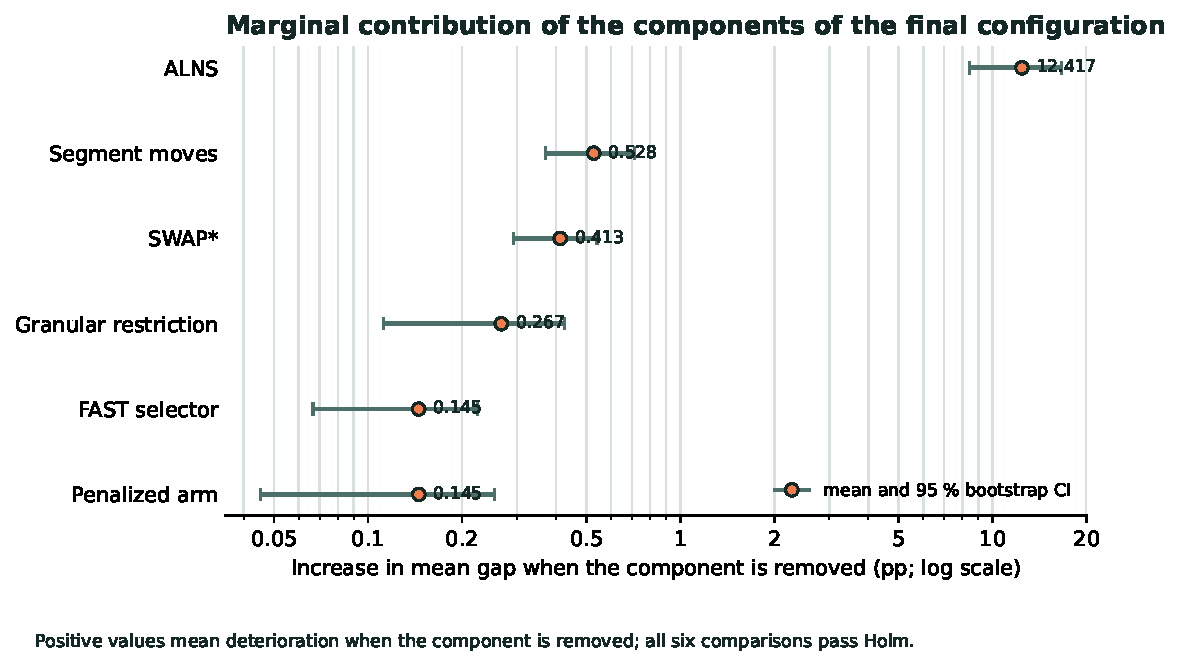
\includegraphics[width=0.82\linewidth]{figuras/F5_component_ablation_forest_en.pdf}
\caption{Increase in the gap when each component is removed (logarithmic scale). All 95\,\% bootstrap
intervals lie above zero.}
\label{fig:forest}
\end{figure}

\begin{ideaclave}[: a hierarchy of mechanisms]
The ALNS is the engine: without it, the gap multiplies by four. Moves between routes (segments and
SWAP*) form a second level. The selector and the penalized arm are refinements of smaller magnitude.
\end{ideaclave}

\subsection{Prospective holdout}
The selector and its thresholds were frozen, with their SHA-256 fingerprint, before running 10 X
instances that had never been observed (\tsl{X-n351-k40} to \tsl{X-n429-k61}). On them the mean gaps
were 4.799\,\% for SENDA, 1.998\,\% for HGS and 0.740\,\% for FILO2. The order between methods is
preserved: the selector works as a rule outside the design instances, but it does not make SENDA the
best solver on X.

% =========================================================================
\section{Case study: an audit that corrected our own results}
\label{sec:caso}

\subsection{What was published}
Version 2 reported on A/B/E a gap of 0.0120\,\% for SENDA versus 0.0059\,\% for HGS, with 3 instances
won by SENDA, 33 ties and 25 losses.

\subsection{How the problem was detected}
When the comparison was repeated in a later campaign, \emph{negative gaps} appeared: SENDA solutions
apparently better than the optimum. Following the alarm of Section~\ref{sec:cvrp}, the routes of
those solutions were counted.

\begin{table}[H]
\centering
\caption{Solutions with cost below the BKS in the project data. None is a legitimate record.}
\label{tab:bks}
\small
\begin{tabular}{@{}llrrl@{}}
\toprule
Instance & BKS ($k$) & Solution & Routes & Verdict \\
\midrule
\tsl{B-n51-k7} & 1032 (7) & 1016 & 8 & uses one vehicle too many \\
\tsl{B-n57-k7} & 1153 (7) & 1140 & 8 & uses one vehicle too many \\
\tsl{E-n30-k3} & 534 (3) & 503 & 4 & uses one vehicle too many \\
\tsl{X-n247-k50}, \tsl{X-n420-k130} & --- & --- & --- & invalid, already excluded in v2 \\
\bottomrule
\end{tabular}
\end{table}

\subsection{The cause}
The program that launched SENDA in the experiments (the \emph{runner}) told it ``free fleet'' even on
A/B/E, and its verification checked coverage and capacity, but not the number of routes. HGS, on the
other hand, was run with the fixed fleet, and FILO2's fleet was verified. In total, 327 SENDA runs
with more than $k$ routes were accepted as valid. A later review of the whole project folder showed
that the same problem affects the A/B/E sensitivity profiles (equalized CPU and parallel portfolio),
whose mean SENDA gaps are also negative, and version 1 of the protocol.

\subsection{The correction}
\begin{enumerate}[leftmargin=1.5em]
\item The published analysis was repeated from the raw data and the same comparison table was
obtained, byte for byte. This confirmed that the reanalysis introduced no changes of its own.
\item The same fleet rule was applied to all methods. In the original data, three instances are left
without any valid SENDA replicate, so those data no longer support the comparison.
\item The experiment was repeated with the corrected runner (fleet equal to $k$), the same budget, the
same seeds and HGS in the same block. With the fleet specified, SENDA respected it in all 630 runs:
the extra vehicle came from the runner, not from the algorithm. That is the result of
Table~\ref{tab:abe}.
\end{enumerate}

\begin{leccion}[: verify everyone equally]
A comparison is fair only if \emph{all} methods are verified with the same rule. Here, a difference in
treatment ---fixed fleet for HGS, free fleet for SENDA--- turned three invalid solutions into ``wins''.
The warning signs were there: families B and E had negative mean gaps. They just had to be looked at
with suspicion. The correction keeps the qualitative conclusion (SENDA is almost optimal on A/B/E),
but changes the magnitude from 0.012\,\% to 0.111\,\% and removes every SENDA win.
\end{leccion}

\begin{reproducir}
Original data: canonical CSV \tsl{f3a1164c85f4\ldots}. Rerun with a verified fixed fleet: contract
\tsl{fef9dd7ee521\ldots}. To repeat the verification with your own results, check in each solution
the number of routes against the fleet of the instance, besides capacity and coverage
(Section~\ref{sec:pruebalo}).
\end{reproducir}

% =========================================================================
\section{Discussion}
\label{sec:discusion}

\paragraph{Two regimes.} On instances of up to one hundred customers, \senda{} is within one tenth of a
point of the BKS in two seconds; HGS is better, but only slightly. On instances of 199 to 428
customers, the gap to HGS and FILO2 grows to between 2 and 3 points. The cascade suggests why: on X,
each arm has little more than one second, and in that time its ALNS barely improves what local search
already achieved (\cgfXd\,\% versus \cgfXc\,\% on the feasible solutions). Time, not construction, is
the bottleneck.

\paragraph{Statistical significance versus practical relevance.} A difference of 0.1\,\% in distance
may be irrelevant or important depending on the operation. When routing is integrated with
three-dimensional loading constraints, time windows and operational rules, those constraints usually
weigh more than differences in pure routing. Quantifying it on the integrated problem is future work;
this document is limited to the classic CVRP.

\paragraph{Limitations.}
(i) The main campaign and the fixed-fleet rerun were executed on different machines. Within each
comparison all methods share a machine, but figures from different sources should not be mixed.
(ii) The holdout contains only 10 instances from one family.
(iii) On X, the cascade uses the A/B/E portfolio and not the X variant of the main campaign
(4.150\,\% versus 4.119\,\%).
(iv) The cascade was measured with the ablation binary, not the confirmatory one.

% =========================================================================
\section{Conclusions}
\label{sec:conclusiones}

\senda{} shows that a single-trajectory-per-run architecture, auditable and without a population,
reaches almost optimal quality on small classic instances: a gap of 0.111\,\% in 2\,s with a verified
fleet, although HGS is equal or better on all of them. On X instances, HGS and FILO2 keep a clear
advantage. The cascade and the ablation agree that the ALNS is the dominant mechanism, that moves
between routes form a second level and that the selector and the penalized arm fine-tune the result.

Methodologically, the project leaves a lesson worth more than any figure: verification must be
uniform, negative gaps are alarms and one's own results must be audited too. Correcting them publicly
does not weaken the work: it makes it credible.

\paragraph{Future work.}
(1) Give the ALNS more effective time on large instances, for example by keeping each arm from
repeating construction and polishing.
(2) Measure the impact of these differences on the integrated problem with three-dimensional loading.
(3) Extend the holdout to other families and up to $n=1000$.

\begin{reproducir}[: artifacts]
\small
\begin{tabular}{@{}p{4.9cm}p{9.6cm}@{}}
Campaign v2 (X, ablation, holdout) & contract \tsl{36f29f1f1795\ldots}, CSV \tsl{f3a1164c85f4\ldots} \\
Fleet correction & contract \tsl{fef9dd7ee521\ldots} \\
Quality cascade & contract \tsl{dd6b8817\ldots}; ablation binary \tsl{4002751d\ldots} \\
Evaluated core and HGS-CVRP & core binary \tsl{d7921fe1\ldots}; HGS-CVRP binary \tsl{4e53fb18\ldots} \\
Figures in this document & data in \tsl{paper/datos/} of this repository \\
Full artifacts & author's archive; shared on request (\tsl{contacto@lattimex.com}) \\
\end{tabular}
\end{reproducir}


% =========================================================================
\section{Try it on your computer}
\label{sec:pruebalo}

The LATTIMEX routing engine uses a later version of SENDA (engine \tsl{1.6.0}): it keeps its
components and adds the parallel portfolio of Section~\ref{sec:portafolio}. The figures in this guide
were measured with binary \tsl{d7921fe1\ldots}, not with the one in the repository. The engine is
published under the MIT license at \texttt{https://github.com/Erick-MF28/lattimex}. In the repository
the core is \tsl{native/senda\_core.cpp}; around it there is a pipeline that turns it into a real
planner: effective capacity, three-dimensional placement of the boxes, fixed-fleet mediation and
unloading plan by door. The comparison programs (HGS-CVRP, FILO2 and the campaign scripts) are not
part of the repository.

\paragraph{1. Install and check the engine.} You need Python 3.10 or later and a C++ compiler (on
Windows \tsl{pip install ziglang} is enough).
\begin{verbatim}
git clone https://github.com/Erick-MF28/lattimex.git
cd lattimex
pip install -r requirements.txt
python -m lattimex build        # compiles the core and the 3D packer
python -m lattimex probe        # deterministic fingerprint: 6457b2dd44660773
python -m unittest discover -s tests/engine
\end{verbatim}
The deterministic fingerprint summarizes a fixed run of 3\,000 iterations. If your build gives the
same fingerprint, your binary computes exactly the same as the one described here, even if the binary
file is not identical byte for byte.

\paragraph{2. See it work on real streets.} The engine builds its own map from OpenStreetMap and
serves it to the graphical interface, the LATTIMEX Planner, which opens in the browser:
\begin{verbatim}
python -m lattimex map --bbox 20.47,-100.52,20.82,-100.22 --name queretaro
python -m lattimex serve        # then open https://lattimex.com/planner
\end{verbatim}
In the Planner's \emph{Guías} (shipments) section, the \emph{Cargar ejemplo} button adds 300 synthetic
deliveries in Querétaro, six vans and five drivers; \emph{Optimizar} computes the routes and the
placement of every box. The computations and the data stay on your computer. The Planner interface is
currently in Spanish.

\paragraph{3. Repeat a comparison fairly.} To measure the core on reference instances (CVRPLIB)
against another solver, obtain that solver from its official source and follow the rules of
Section~\ref{sec:evaluar}:
\begin{enumerate}[leftmargin=1.5em]
\item the same wall clock for all methods, on the same machine and on a single thread;
\item at least 10 replicates with different seeds per instance;
\item the same fleet for everyone, fixed in advance;
\item an independent verifier that recomputes distance, capacity, coverage and number of routes;
\item paired comparisons per instance and correction for multiple comparisons (Holm).
\end{enumerate}
A negative gap against the best known solution is almost always an alarm: check the fleet and the
rounding of distances first.

\begin{ideaclave}
Open source lets anyone repeat the measurements. If your results differ from those in this guide,
write to us: a well-documented discrepancy is a contribution.
\end{ideaclave}

\bibliographystyle{plain}
\bibliography{referencias_en}

% =========================================================================
\appendix
\section{Glossary}
\label{app:glosario}
\begin{description}[leftmargin=0pt,font=\bfseries]
\item[BKS] Best known solution of a reference instance.
\item[Gap] Relative difference between the cost obtained and the BKS (equation~\ref{eq:gap}).
\item[Local optimum] Solution that no move of a given neighborhood can improve.
\item[Replicate] Independent run with another seed. Here 10 per instance are used.
\item[Arm] One independent search within a trial; the portfolio has two or three.
\item[Wall-clock time] Real elapsed time, measured with a clock; distinct from CPU time.
\item[Construction] Procedure that generates the first complete solution.
\item[Local search] Repeated application of small changes that improve the solution.
\item[Granular restriction] Limiting moves to pairs of nearby customers.
\item[ALNS] Adaptive large neighborhood search: destroys and repairs parts of the solution with
operators whose weights learn.
\item[Simulated annealing] Rule that accepts worse solutions with a probability that decreases over
time.
\item[Regret-2] Repair that first inserts the customer that would lose the most if left for later.
\item[SWAP*] Exchange of two customers between routes, each at its best position in the other route.
\item[Portfolio] SENDA configuration evaluated on A/B/E: base branch, FAST branch and penalized arm.
\item[Penalized arm] Search that tolerates temporary capacity excesses in exchange for a penalty.
\item[Contract] Frozen file with code, parameters, instances and tests, identified by its SHA-256
fingerprint.
\item[Holdout] Set of instances reserved and not observed during design.
\item[Holm] Correction for multiple comparisons that controls the family-wise error.
\item[Big-$O$] Notation that describes how the number of operations of an algorithm grows with the
size of the input (Section~\ref{sec:complejidad}).
\end{description}

\section{Literal rule of the FAST selector}
\label{app:selector}

\begin{algorithm}[H]
\caption{Additional configuration chosen by FAST from $\phi(I)$}
\begin{algorithmic}[1]
\Require $n$, $k$, load pressure $\ell$, demand CV $c_q$, radial CV $c_r$, angular concentration $\alpha$, density $\eta$
\If{$n<150$}
  \IfReturn{$n\ge70$}{\tsl{granular\_k25}}
  \If{$60\le n<70$}
    \IfReturn{$\eta\ge0.0085$ or $\alpha<0.35$}{\tsl{large\_destroy\_k25}}
    \IfReturn{$\alpha\ge0.80$}{\tsl{long\_10k\_k25}}
    \IfReturn{$k\ge10$}{\tsl{granular\_k40}}
    \IfReturn{$c_q<0.50$}{\tsl{long\_10k\_k25}}
    \State \Return \tsl{baseline}
  \EndIf
  \IfReturn{$45\le n\le65$ and $\ell<0.93$ and $c_q<0.50$}{\tsl{medium\_destroy\_k25}}
  \State \Return \tsl{baseline}
\EndIf
\IfReturn{$c_q\ge0.50$ and ($n\le245$ or $k\ge70$)}{\tsl{large\_destroy\_k25}}
\IfReturn{$k\le16$ and [($c_q<0.30$ and $c_r<0.38$) or ($c_q<0.70$ and $\alpha\ge0.88$)]}{\tsl{granular\_k25}}
\IfReturn{$k\ge55$ and $c_q\ge0.45$ and $\alpha\ge0.90$}{\tsl{granular\_k25}}
\IfReturn{$n\ge300$ and $c_q\ge1.0$}{\tsl{baseline}}
\State \Return \tsl{long\_10k\_k25}
\end{algorithmic}
\end{algorithm}

\noindent If the chosen configuration is \tsl{baseline}, the trial runs only the base branch and its
penalized arm. Otherwise it runs the base branch, the chosen branch and the penalized arm of the
latter.

\section{Errata with respect to version 2}
\label{app:errata}
\begin{itemize}[leftmargin=1.5em]
\item \textbf{A/B/E}: ``SENDA 0.0120\,\% versus HGS 0.0059\,\%, 3/33/25, $p=0.00406$'' is replaced by
``SENDA 0.111\,\% versus HGS 0.004\,\%, 0/37/23, $p=2.4\times10^{-7}$ (60 pairs, verified fixed
fleet)''.
\item \textbf{Verification}: the statement that the fleet of every solution was verified was not true
for SENDA in campaign v2; it was corrected in the rerun.
\item \textbf{Gates}: with the verified fleet, the gate of the A/B/E comparison of campaign v2 fails;
those of X, ablation and holdout pass unchanged.
\item \textbf{Per-instance map figure}: the three cells favorable to SENDA corresponded to solutions
with $k+1$ vehicles (Figure~\ref{fig:abe}).
\end{itemize}

\end{document}
